\section{Rezultatai}



\subsection{Difuzijos srovės palyginimas su dreifo srove}

\begin{figure}[H]
  \centering
    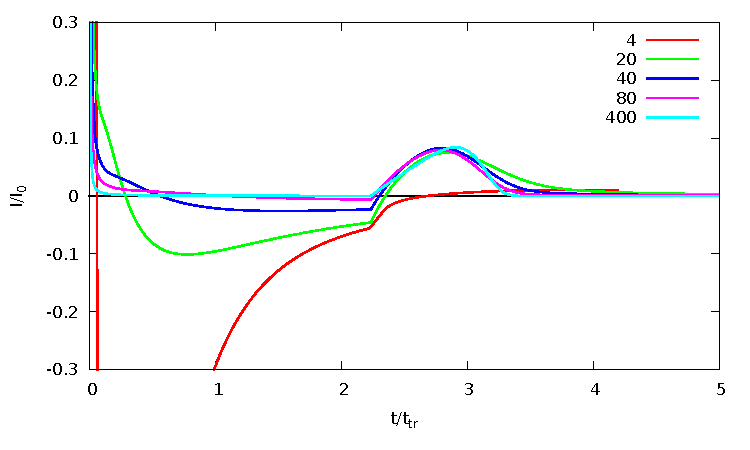
\includegraphics{./media/pdf/diff_drift.pdf}
  \caption{Photo-CELIV kinetikos su skirtingais $eU/kT$ esant paviršinei krūvininkų generacijai $\alpha d = 100$}
  \label{fig:comp}
\end{figure}

Norėdami įvertinti difuzijos įtaką photo-CELIV signalams įsivedėme santykį $eU/kT$. Akivaizdu, jog mažinant šį santykį difuzijos įtaka didės (žr. \ref{fig:comp} pav.). Esant kambario temperatūrai šis koeficientas lygus $40$. Tolesniuose skaičiavimuose naudojama būtent pastaroji vertė.
Paveiksliuke \ref{fig:comp} matomos neigiamos kinetikų dalys atsirandančios dėl difuzijos. Esant dideliam krūvininkų tankio gradientui, dėl Demberio efekto greitesnieji krūvininkai yra paskumiami į bandinio vidų. Prie kontakto likę krūvininkai sparčiai rekombinuoja ir sukuria kitos krypties krūvininkų gradientą. Greitesnieji krūvininkai ima judėti atgal link kontakto, sukurdami neigiamą srovę. Platesnis pastarojo reiškinio aprašymas pateiktas priede \ref{app:negative_current}.

\subsection{Photo-CELIV srovės kinetikos} 
\begin{figure}[H]
    \centering
	\subfloat[$\alpha d = 0.1$]{
		\label{fig:transient_ad=0.1}
		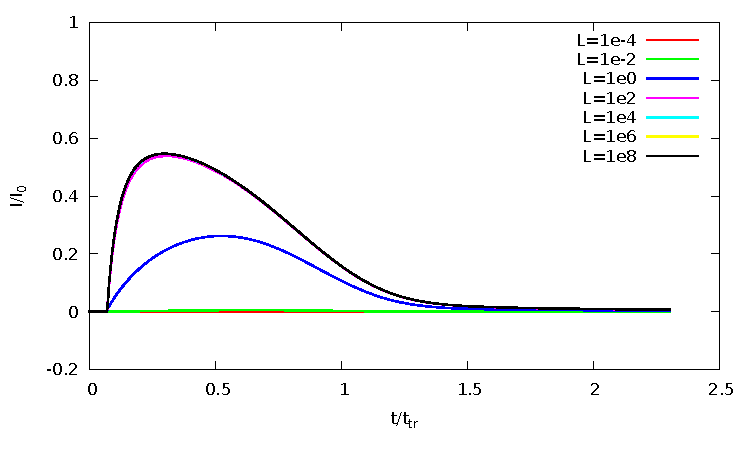
\includegraphics[width=0.5\textwidth]{./media/pdf/transient_ad01.pdf}
		}
	\subfloat[$\alpha d = 10$]{
		\label{fig:transient_ad=10}
		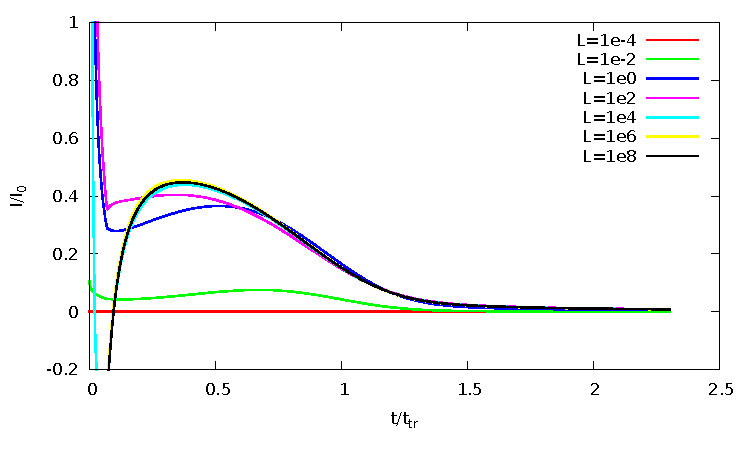
\includegraphics[width=0.5\textwidth]{./media/pdf/transient_ad10.pdf}
		}
  \caption{Photo-CELIV kinetikų pavidalo priklausomybė nuo šviesos intensyvumo, priklausomai nuo sugerties profilio, esant minimaliai užlaikymo trukmei $t_{delay} = 0.07t_{tr}$ ir įskaičius difuziją}
  \label{fig:transients}
\end{figure}

Įskaičius difuziją photo-CELIV srovės kinetikos kokybiškai keičiasi keičiant sugerties profilį $\alpha d$. Tai iliustruota \ref{fig:transients} paveiksliuke. Matome, jog didinant šviesos intensyvumą kinetikos įsisotina ir nebekinta.

\subsection{Difuzijos įtaka photo-CELIV srovės sotinimuisi}
\label{page:saturation}
\begin{figure}[H]
  \centering
    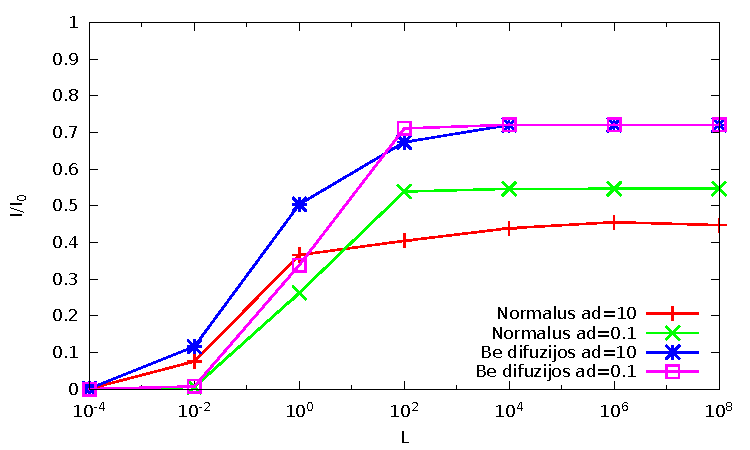
\includegraphics{./media/pdf/semilogsaturation.pdf}
  \caption{Photo-CELIV kinetikų maksimumo srovės vertės sotinimasis nuo šviesos intensyvumo, priklausomai nuo difuzijos ir sugerties profilio, esant minimaliai užlaikymo trukmei $t_{delay} = 0.07t_{tr}$}
  \label{fig:saturation}
\end{figure}

Rekombinacijos įvertinimui eksperimentuose dažniausiai naudojama photo-CELIV srovės soties vertė, kai nėra užlaikymo tarp šviesos impulso ir ištraukiančios įtampos impulso. Skaičiavimuose įtraukėme pastovią užlaikymo trukmę $t_{delay}$, dėl priežasties parodytos \ref{page:limits} skyrelyje. Nustatėme intensyvumo parametro vertę, kuriai esant kinetika yra įsisotinusi. Vėlesniuose skaičiavimuose naudojome parametrą $L=10^{10} L_0$. Pagal \cite{juška:155202} soties vertė, esant bimolekulinei Lanževeno rekombinacijai turėtų artėti į $I_0$. Tačiau suskaičiuotuose rezultatuose (žr. \ref{fig:saturation} pav.) matome, jog srovė sotinasi į vertę, mažesnę už $I_0$. Toliau parodyta, kad ši vertė priklauso nuo užlaikymo trukmės.
Taip pat matome, jog neįskaičius difuzijos, soties vertė nepriklauso nuo krūvininkų pradinio pasiskirstymo, kinta tik įsisotinimo greitis.
Įskaičius difuziją, srovės soties vertė ima priklausyti nuo $\alpha d$.
Suskaičiuoti tarpiniai rezultatai su $\alpha d$ intervale $[0.1 , 10]$ patenka tarp kraštinių kreivių ir dėl aiškumo nepavaizduoti.

\subsection{Užlaikymo trukmės įtaka photo-CELIV srovės sotinimuisi}

\begin{figure}[H]
  \centering
	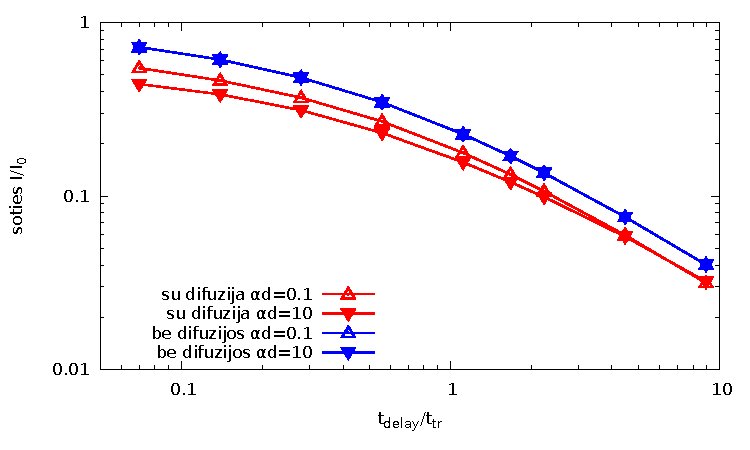
\includegraphics{./media/pdf/delays.pdf}
  \caption{Photo-CELIV srovės kinetikų soties vertės priklausomybės nuo užlaikymo trukmės $t_{delay}$}
  \label{fig:delays}
\end{figure}

Norėdami įvertinti užlaikymo trukmės įtaką photo-CELIV srovės soties vertei atlikome skaičiavimus su skirtingomis užlaikymo trukmėmis, kurių rezultatai pavaizduoti \ref{fig:delays} paveiksliuke.

Pastebime, jog rekombinacijos įvertinimas pagal soties reiškinį jautrus užlaikymo laikui $t_{delay}$. Taip pat šie rezultatai dar kartą parodo, jog veikiant difuzijai kinetikų soties vertė priklauso nuo krūvininkų sugerties profilio. Akivaizdžiai matomas ir bendras soties srovės sumažėjimas dėl difuzijos.

Aptarkime, kuomet Photo-CELIV srovės maksimumo vertė yra proporcinga krūvininkų kiekiui bandinyje. Jei nėra difuzijos ir krūvininkų ištaukimo metu rekombinacijos įtakos krūvininkų kiekiui galime nepaisyti, tai $I_{max} \sim n$, čia $n$ -- krūvininkų tankis. Šiuo atveju remdamiesi krūvininkų tankio lygties su įskaityta rekombinacija sprendiniu $$ n(t) = \frac{1}{\frac{1}{n_0} + \beta t} $$ galime teigti, jog atidėję $I_{max}$ nuo užlaikymo trukmės $t_{delay}$ logaritminiame mastelyje turime gauti tiesę, kurios polinkis $-1$, jei laikysime $\frac{1}{n_0} \rightarrow 0$. Čia $n_0$ -- pradinis krūvininkų tankis.
Šio teiginio patikrinimui \ref{fig:delays} paveiksliuke nubrėžta tiesė, kurios polinkis $-1$.

\subsection{Rekombinacijos įtaka pradinėms sąlygoms}
\begin{figure}[H]
  \centering
	\subfloat[$\alpha d = 0.1$]{
		\label{fig:recomb_ad=0.1}
		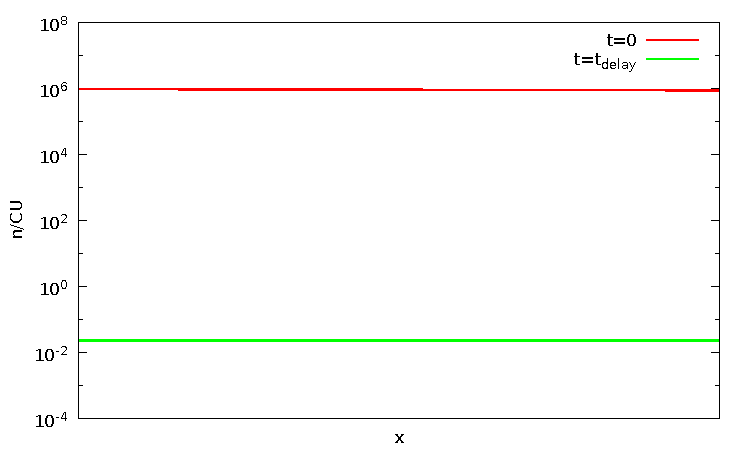
\includegraphics[width=0.5\textwidth]{./media/pdf/recomb_ad01.pdf}
		}
	\subfloat[$\alpha d = 10$]{
		\label{fig:recomb_ad=10}
		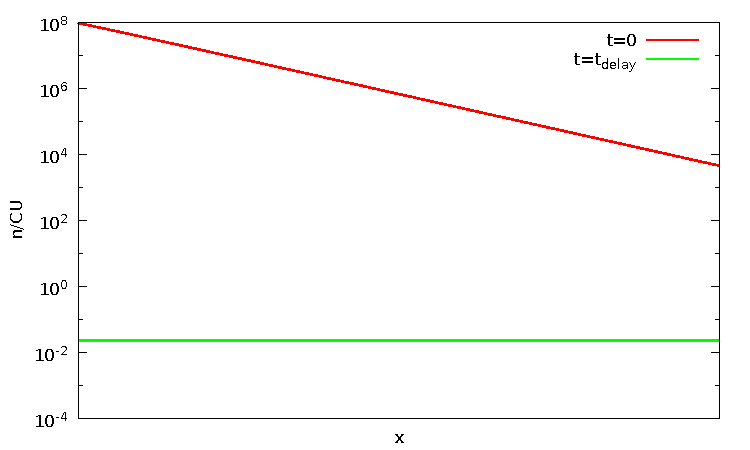
\includegraphics[width=0.5\textwidth]{./media/pdf/recomb_ad10.pdf}
		}
  \caption{Dėl rekombinacijos susilyginančios pradinės sąlygos per užlaikymo trukmę $t_{delay} = 0.07t_{tr}$, kai nėra difuzijos.}
  \label{fig:recomb}
\end{figure}

Dėl rekombinacijos, esant soties sąlygas atitinkančiam šviesos intensyvumui, neįskaitant difuzijos, po užlaikymo laiko $t_{delay}$ bandinyje, nepriklausomai nuo pradinio apšvietimo tipo nusistovi vienodi krūvininkų pasiskirstymai (žr. \ref{fig:recomb} pav.).
Dėl šio reiškinio, photo-CELIV srovės kinetikų soties vertės, kai nėra difuzijos, sutampa (žr. \ref{fig:delays} pav.).

\subsection{Judrio vertės skaičiavimai}

\begin{figure}[H]
  \centering
	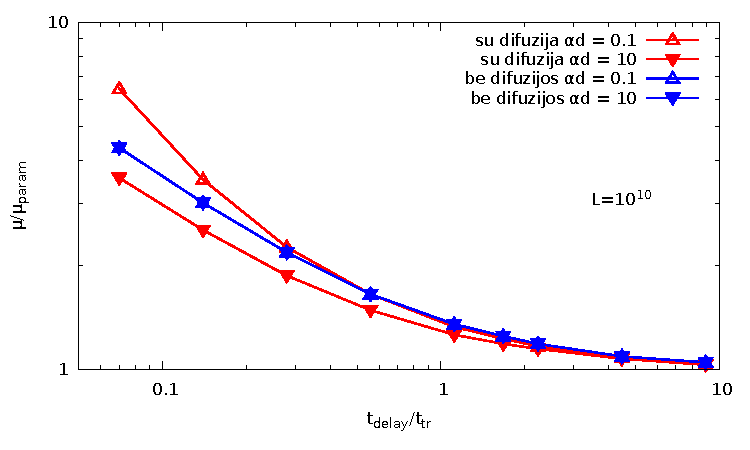
\includegraphics{./media/pdf/log_mobility.pdf}
  \caption{Krūvininkų judrio skaičiavimo pagal \eqref{eq:judris} formulę rezultatų priklausomybė nuo $t_{delay}$}
  \label{fig:mobility}
\end{figure}

Pagal \eqref{eq:judris} formulę skaičiuojant krūvininkų judrį iš įsisotinusių srovės kinetikų maksimumų gaunama krūvininkų judrio priklausomybė nuo užlaikymo trukmės pavaizduota \ref{fig:mobility} paveiksliuke. Anksčiau panašūs rezultatai buvo aiškinami krūvininkų prilipimu \cite{juška:2004290}. Tačiau šioje simuliacijoje krūvininkų prilipimas nėra įskaitomas, taigi egzistuoja kitos priežastys šiam kitimui. Viena iš priežasčių yra krūvininkų kiekio pakitimas dėl rekombinacijos bandinyje paliktame laikui $t_{delay}$. Ankstesniuose darbuose \cite{juška:155202} parodyta, jog dėl pradinio krūvininkų kiekio \eqref{eq:judris} formulėje reikia įskaityti pataisos koeficientą. Antroji priežastis yra krūvininkų pasiskirstymo pakitimas dėl rekombinacijos. Taigi tiksliam judrio įvertinimui reikia suskaičiuoti papildomą pataisos koeficientą, priklausantį nuo užlaikymo trukmės ir rekombinacijos koeficiento.

Difuzijos įtaką šiems rezultatams galime nagrinėti atskirdami srovės komponentes. Esant paviršiniam pasiskirstymui $\alpha d = 10$ dėl didelio krūvininkų tankio gradiento greitesnieji krūvininkai yra pastumiami į bandinio gilumą. Likusieji greitai rekombinuoja dėl didelio tankio ir tokiu būdų susiformuoja krūvininkų tankio gradientas į priešingą pusę. Tuo pačiu difuzinės srovės kryptis pasikeičia. Ši srovė laipsniškai slopsta. Šio proceso sukurta kinetika matoma \ref{fig:comp} paveiksliuke. Prie tokios komponentės pridėję photo-CELIV signalą (žr. \ref{fig:celiv_example} pav.) gausime $t_{max}$ padidėjimą, taigi suskaičiuotasis krūvininkų judris medžiagoje sumažės. Esant tūriniam pasiskirstymui $\alpha d = 0.1$ nedidelė difuzinės srovės komponentė, kuri veikia į bandinio gilumą, sumažina $t_{max}$, taigi padidina išmatuotą kruvininkų judrį.
